% !TEX root = main.tex

\chapter{Interazioni tra Radiazione e Materia}

In questo capitolo studieremo come interagiscono con la materia ioni, elettroni, positroni, fotoni, neutroni.

\section{Interazioni Ioni-Materia}

\begin{figure}
\centering
	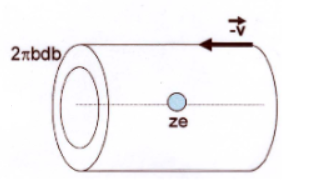
\includegraphics[keepaspectratio]{figs/rutherford.png}
	\caption{Applicazione del teorema di Gauss nel sistema di riferimento dello ione}
	\label{fig:rutherford}
\end{figure}


Ai regimi di energia che interessano a noi gli ioni interagiscono prevalentemente con gli elettroni della materia su cui incidono, potenzialmente ionizzandola. Si usano come ioni proiettili atomi completamente ionizzati quali $H^+$, $He^{2+}$ e $C^{6+}$.
Inoltre l'energia dello ione è dell'ordine del MeV, mentre quella dell'elettrone ordine eV, dunque nella schematizzazione che segue considereremo fermo l'elettrone.
Siccome lo ione è molto più massivo dell'elettrone possiamo metterci nel suo sistema di riferimento e considerarlo imperturbato nel corso dell'interazione. 

\begin{equation}
\Delta p_e=\int Fdt = e\int Edt = \frac {e}{v}\int E \mathrm{d}x
\end{equation}

Prendendo un cilindro immaginario intorno allo ione ed applicando il teorema di Gauss ottengo

\begin{equation}
\Phi(E)=2\pi b \int E \mathrm{d}x =\frac{Ze}{\epsilon_0}
\end{equation}

Dove $b$ è il raggio di base del cilindro.\\
Dalla precedente equazione si ricava:

\begin{equation}
\int E \mathrm{d}x= \frac{Ze}{2\pi b \epsilon_0}
\end{equation}

Sostituendo nell'espressione per la variazione della quantità di moto dell'elettrone ottengo:

\begin{equation}
\Delta p_e=\frac{Ze^2}{2\pi\epsilon_0vb}
\end{equation}

Da cui l'energia cinetica totale trasferita da ione a elettrone è:

\begin{equation}
\Delta K_{I,e}=\frac{\Delta p_e^2}{2m_e}=(\frac{Ze^2}{2\pi\epsilon_0vb})^2\frac{1}{2m_e}
\end{equation}

Verifichiamo ora che le approssimazioni fatte siano ragionevoli. Prendiamo ad esempio uno ione idrogeno incidente con impulso iniziale di $100 MeV/c$. Per esso $E\simeq m$ dunque $\beta\simeq\frac{p}{m}=0,1$.

\begin{equation}
 |\Delta p_I|=|\Delta p_e|=\frac{Ze^2}{2\pi\epsilon_0vb}=\frac{2Z\alpha}{\beta b}\cdot(\hbar c)^mc^n  
\end{equation}

Dall'equazione $p=\frac{E}{c}$ per l'impulso di una particella non massiva sappiamo che le dimensioni dell'impulso sono $[p]=\frac{E\cdot T}{L}$. Le dimensioni corrette si ottengono nell'equazione precedente scegliendo quindi $m=1$ e $n=-1$.

\begin{equation}
|\Delta p_I|=\frac{2\cdot 200 MeV\cdot fm}{137 \cdot 0,1 \cdot c \cdot b}
\end{equation}

A noi interessa capire per quali valori di $b$ vale la approssimazione $\frac{\Delta p_I}{p_I}<<1$. 
Con i dati che abbiamo noi ciò si traduce in $\Delta p_I<<100 MeV/c$ ovvero 

\begin{equation}
\frac{29 fm}{b}<<100
\end{equation}

Che si traduce come condizione su $b$ in:

\begin{equation}
b>>0,3 fm
\end{equation}

E ciò si verifica praticamente sempre. Ovvero lo ione per essere perturbato nel suo moto dovrebbe avvicinarsi a meno di $0,3 fm$ dal nucleo, cosa altamente improbabile.

\emph{Nota: il trasferimento di impulso è inversamente proporzionale alla velocità dello ione! Infatti più esso è lento, più tempo trascorre vicino all'elettrone, trasferendogli impulso.}

Bibliografia: \cite{Longo}

\section{Bethe-Block}

La formula di Bethe-Block descrive la perdita di energia per unità di spazio percorso per una particella massiva carica che fa ionizzazione in un materiale. Tale formula si dimostra\footnote{\texttt{https://userswww.pd.infn.it/~carlin/riv/Slides/parte1.pdf}} essere:

\begin{equation}
-\frac{dE}{dx}=4\pi N_A\frac{Z\rho}{A}r_e^2m_ec^2\frac{z^2}{\beta^2}(\ln\frac{2m_ec^2\beta^2\gamma^2}{I}-\beta^2-\frac{\delta(\gamma)}{2})
\end{equation}

Nel range di energie che interessano a noi ($\beta\gamma<2$) la funzione è approssimabile nella formula $\frac{1}{\beta^2}$ ovvero all'aumentare della velocità la perdita di energia scende con il suo quadrato. Come avevamo visto dalle considerazioni nel paragrafo precedente se lo ione incidente è più lento, perderà più energia nell'unità di percorso. Al di là del tipo di materiale in cui sto incidendo, in generale, per $\beta\gamma$ dell'ordine dell'unità ho che $-\frac{1}{\rho}\frac{dE}{dx}\simeq2MeV g^{-1}cm^{2}$.
Il fatto che lavoriamo ad energie più basse si vede perché imponendo $\beta\gamma=3$ si ottiene un energia cinetica dell'ordine dei $5 GeV$, molto maggiore di quelle effettivamente usate in medicina.

\begin{figure}
\centering
	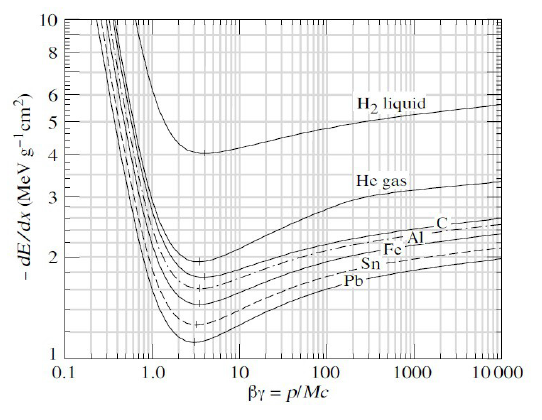
\includegraphics[width=10cm, keepaspectratio]{figs/bethe.png}
	\caption{Grafico della formula di Bethe-Block. Si osserva il primo tratto di discesa in cui domina il termine $\frac{1}{\beta^2}$, il minimo a $\beta\gamma=2m_0c^2$ e il seguente tratto di risalita.}
	\label{fig:bethe}
\end{figure}



\newpage

\section{Stopping Power e Linear Energy Transfer (LET)}

Abbiamo visto prima l'andamento della Bethe Block e l'intervallo di nostro interesse. Fissata una velocità iniziale, il moto della particella in esame attraverso un certo materiale può solo rallentare. Ovvero la particella può solo muoversi a sinistra nel grafico e quindi rimarrà sempre nel regime $\frac{1}{\beta^2}$. In pratica con lo svolgersi del processo la particella diminuirà $\beta\gamma$ e aumenterà $\frac{dE}{dx}$, fino ad un massimo che corrisponderà al range totale della particella, dopo il quale essa ha perso tutta l'energia. L'integrale di $\frac{dE}{dx}$ da 0 al range deve restituire dunque l'energia iniziale della particella. 
Questo $\frac{dE}{dx}$ rappresenta lo stopping power, ovvero l'energia rilasciata dalla particella. Essa non sempre coincide con l'energia assorbita dal paziente. La quantità che misura l'energia assorbita dal paziente è il LET. La prima differenza quantitativa tra le due grandezze è che il LET va come $\frac{1}{\beta^{2*0,82}}$ e la formula empirica che lo descrive (valida nel range di energie trattate nella fisica medica) è:

\begin{equation}
LET=\frac{L_0Z^2}{(K/m)^{0,82}} \qquad \qquad L_0(acqua)=0,12 \frac{keV}{\mu m}
\end{equation}

Passiamo al calcolo del Range \cite{Amaldi}:

\begin{equation}
R=\int_{K_0}^0 \frac{dK}{-|{\frac{dE}{dx}|}} =\int_0^{K_0} \frac{dK}{LET} = \int_0^{K_0} \frac{dK (K/m)^{0,82}}{L_0Z^2}  
\end{equation}

\begin{equation}
R(K)=R^*\frac{A}{Z^2}(K/m)^{1,82} \qquad \qquad R^* = 425 cm
\end{equation}

\emph{Nota: queste considerazioni valgono per $K/m<$0,4. Nel caso di protoni ciò si traduce in $K<400 MeV$.}

Questa formula per $R$ può essere intesa come funzione di $K$. Ovvero esprime il cammino che resta alla particella in esame se ha energia cinetica $K$. Posso anche esprimere il $LET$ in funzione del cammino che resta: basta invertire la relazione tra $R$ e $K$ e sostituire nella formula del LET. Si ottiene:

\begin{equation}
LET(R)=L_0Z^{1,1}A^{0,45}(R^*/R)^{0,45}
\end{equation}

Ora, considerando che $R$ è il cammino restante alla particella e $x=R_0-R$ e la posizione reale, l'equazione precedente viene riformulata:

\begin{equation}
LET(x)=L_0Z^{1,1}A^{0,45}(\frac{R^*}{R_0-x})^{0,45}
\end{equation}

\textbf{Prima Esercitazione}

\emph{Graficare il range in funzione dell'energia cinetica e il LET in funzione della posizione per protoni, particelle alfa e nuclei di carbonio in acqua.}

L'espressione analitica di LET(x) presenta un asintoto. Nella realtà esso viene scavalcato, perché il fascio di particelle incidenti ha sempre un'incertezza sulla sua energia e sulla sua distribuzione spaziale. Solo un fascio puramente monocromatico avrebbe un andamento asintotico. 

Il massimo assunto di LET(x) deve essere di $20 eV/mm$ per distruggere direttamente il DNA tumorale. Se si vuole solo creazione di radicali liberi bastano energie anche minori.

L'adroterapia è convenzionalmente a basso LET, col solo obiettivo di creare radicali liberi. 

Il plot reale dell'andamento di LET(x) è detto curva di Bragg. Confrontando la curva di Bragg di un protone con quella di un nucleo di carbonio facciamo le seguenti osservazioni:

\begin{itemize}
\item Il picco di Bragg degli ioni carbonio è più stretto e più alto di quello dei protoni
\item Il carbonio presenta una coda dopo il picco che risulta pericolosa
\end{itemize}

\begin{figure}
\centering
	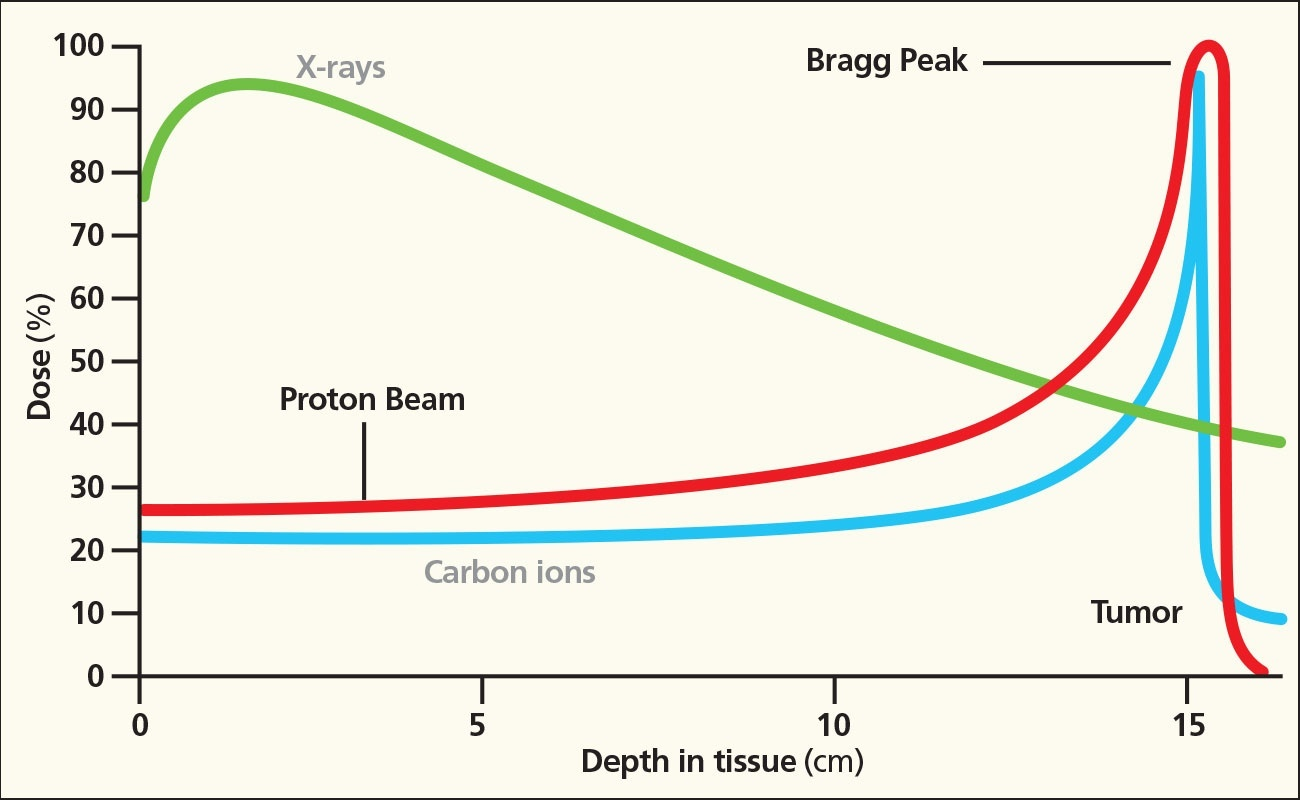
\includegraphics[width=10cm, keepaspectratio]{figs/bragg.jpg}
	\caption{Dose relativa in funzione della penetrazione per fotoni, protoni e carbonio. Il grafico è rappresentativo dell'andamento di LET(x) a meno di una costante. Immagine da scripps.org}
	\label{fig:bragg}
\end{figure}


\section{Scattering Multiplo - Ioni-Nuclei}

Fino ad ora abbiamo osservato il caso in cui lo ione interagisca con gli elettroni del materiale e ci sia un trasferimento di energia per ionizzazione.
Nel caso in cui però lo ione interagisca con il nucleo invece di uno scambio di energia ci sarà una variazione di quantità di moto che si concretizza in una variazione di direzione per lo ione. Esso verrà deviato nel suo percorso. Siccome avvengono tante di queste interazioni si parla di \emph{Scattering Multiplo}. 
Il risultato finale è che un fascio collimato fuoriesce con una distribuzione gaussiana con deviazione standard:

\begin{equation}
\sqrt{\sigma_{\theta}^2}=\frac{z}{\beta p}\sqrt{\frac{x}{X_0}}
\end{equation}

Dove $x$ è lo spessore percorso, $X_0$ una costante del materiale.

\emph{Nota: Il multiple scattering è la vera ragione dello smussamento dell'asintoto di $LET(X)$. Infatti se ad energie diverse corrisponde un angolo finale diverso ciò vuol dire che il range (proiettato su X) è diverso per ogni energia e dunque si spalma intorno al massimo. Da qui anche il motivo per cui il carbonio ha un massimo più definito: subisce meno multiple scattering.}

\begin{figure}
\centering
	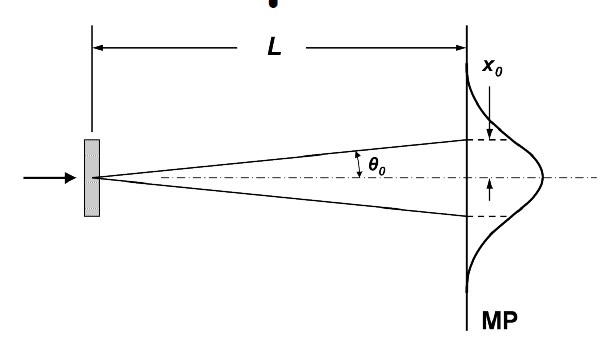
\includegraphics[width=10cm, keepaspectratio]{figs/multiplescattering.png}
	\caption{Rappresentazione dell'effetto del Multiple Scattering. L'angolo in uscita ha una distribuzione di tipo gaussiano.}
	\label{multiplescattering}
\end{figure}

\textbf{Seconda Esperienza}

\begin{itemize}
\item \emph{Stimare CSDA (range reale, non proiettato) e range proiettato in acqua per particelle alfa e protoni con energia cinetica tra $1$ e $10$ $MeV$.}
\item \emph{Stimare la quantità di teflon, ferro e piombo necessarie a fermare particelle alfa e protoni di energie $1$, $5$ e $10$ $MeV$.}
\end{itemize}

\section{Interazioni Elettroni-Materia}

Un elettrone che incide sul bersaglio può interagire fondamentalmente in tre modi. Il primo è per ionizzazione come gli ioni. La formula di Bethe Block va aggiustata per questioni relativistiche e diventa

\begin{equation}
-\frac{dE}{dx}=0,306 N_A\frac{Z\rho}{A}\frac{1}{\beta^2}\ln(\frac{1,16m_ec^2\beta^2}{2I}) MeV/cm\qquad per \beta<0,5
\end{equation}

\begin{equation}
-\frac{dE}{dx}=0,153 N_A\frac{Z\rho}{A}\frac{1}{\beta^2}\ln(\frac{E(E+m_ec^2)^2\beta^2}{2I^2m_ec^2}) MeV/cm \qquad per \beta\simeq 1
\end{equation}

Se invece l'elettrone interagisce con i nuclei del materiale può avvenire multiple scattering (molto più intenso che per gli ioni data la leggerezza degli elettroni) o Brehmsstrahlung. 
Infatti un elettrone che viene deviato nel suo moto da un nucleo, emette radiazione. La potenza dell'emissione è data da:

\begin{equation}
W(\theta)=\frac{q^2a^2sin^2\theta}{4\pi\epsilon_{0}c^3}
\end{equation}

\begin{figure}
\centering
		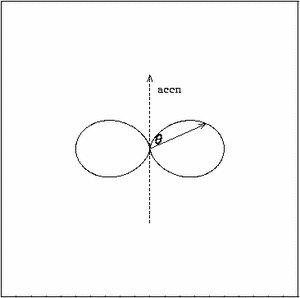
\includegraphics[width=6cm, keepaspectratio]{figs/brehm.png}
		\caption{Andamento dell'energia irradiata in funzione dell'angolo con la direzione del moto}
         \label{brehmtheta}
\end{figure}

Dove $\theta$ è l'angolo tra la direzione del moto dell'elettrone e la direzione della radiazione irradiata.

L'effetto sull'energia dell'elettrone è dato dalla seguente equazione:

\begin{equation}
-\frac{dE}{dx}=\frac{E}{X_0}
\end{equation}

Con soluzione

\begin{equation}
E(x)=E(0)e^{-x/X_0}
\end{equation}

dove 

\begin{equation}
X_0\simeq\frac{A}{N_A Z^2 \rho}\frac{1}{4 \alpha_{em}r_e^2 \ln(\frac{184}{Z^{1/3}})}
\end{equation}

Allo spettro continuo prodotto dalla radiazione di frenamento si possono sommare inoltre delle righe caratteristiche dovute ad un secondo processo: la radiazione di guscio K. 
Questo processo si verifica quando il fotone emesso dall'elettrone frenato ionizza gli atomi del bersaglio colpendo non gli elettroni di valenza ma quelli più vicini al nucleo. Quando ciò succede gli elettroni esterni possono scendere ai livelli più vicini al nucleo emettendo radiazione X. Si parla di $K_{\alpha}$ quando si indica la radiazione emessa da un elettrone che passa da $n=2$ a $n=1$, mentre si parla di $K_{\beta}$ quando si vuole indicare radiazione emessa da un elettrone che scende da $n=3$ a $n=1$. Questa radiazione è monocromatica, pur essendo in origine generata da uno spettro continuo.

Lo spettro totale è mostrato nella figura (\ref{brehmspect})

\begin{figure}
\centering
		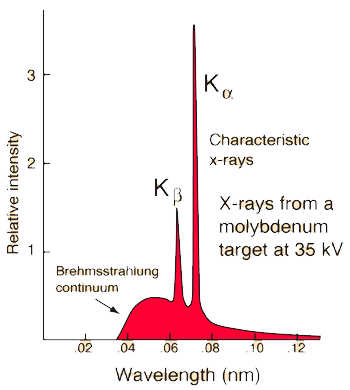
\includegraphics[width=7cm, keepaspectratio]{figs/Spettroxrays.png}
		\caption{Spettro della radiazione risultante, dato da Brehmsstrahlung e radiazione di guscio K}
         \label{brehmspect}
\end{figure}

Notare che la lunghezza d'onda più spostata a sinistra coincide con l'energia iniziale dell'elettrone.

\emph{Nota: per elettroni proiettili la radiazione di frenamento domina sulla ionizzazione solo se $E>\frac{800 MeV}{Z}$. Nel corpo umano $Z\sim6$ dunque la radiazione di frenamento domina come $LET$ solo se $E>133 MeV$ che è enorme per le energie mediche. Quindi nei nostri interessi per gli elettroni nei pazienti domina sempre la ionizzazione.}

A causa dell'intensità del multiple scattering che porta alla dispersione degli elettroni, non ha più senso proiettare il $LET$ sull'asse $x$. La distribuzione viene tutta concentrata all'inizio perché proiettando concentro lì tutte le direzioni diverse da quella $x$.
Questa distribuzione del $LET$ ha un applicazione notevole: utile per i tumori della cute. Si spalma una pomata contenente $^{118}Re$ (\emph{Brachiterapia}\cite{Brachioterapia}) o si spara direttamente con un LINAC sulla zona interessata, che magari è la parete di un organo sensibile da cui è difficile asportare il tumore (Intra Operative Radio Therapy (IORT)\cite{Intraoperative_probes}), ad esempio le pareti dell'aorta.
Per lo spettro completo (Brehmsstrahlung + radiazione caratteristica) guardare la Tesina.
Assumendo un ascissa curvilinea che segue il percorso da multiple scattering degli elettroni e graficando il $LET$ in funzione di tale ascissa osservo un grafico identico a quello del protone proiettato. Tale ascissa curvilinea è detta $CSDA$.

\begin{figure}
\centering
		%% 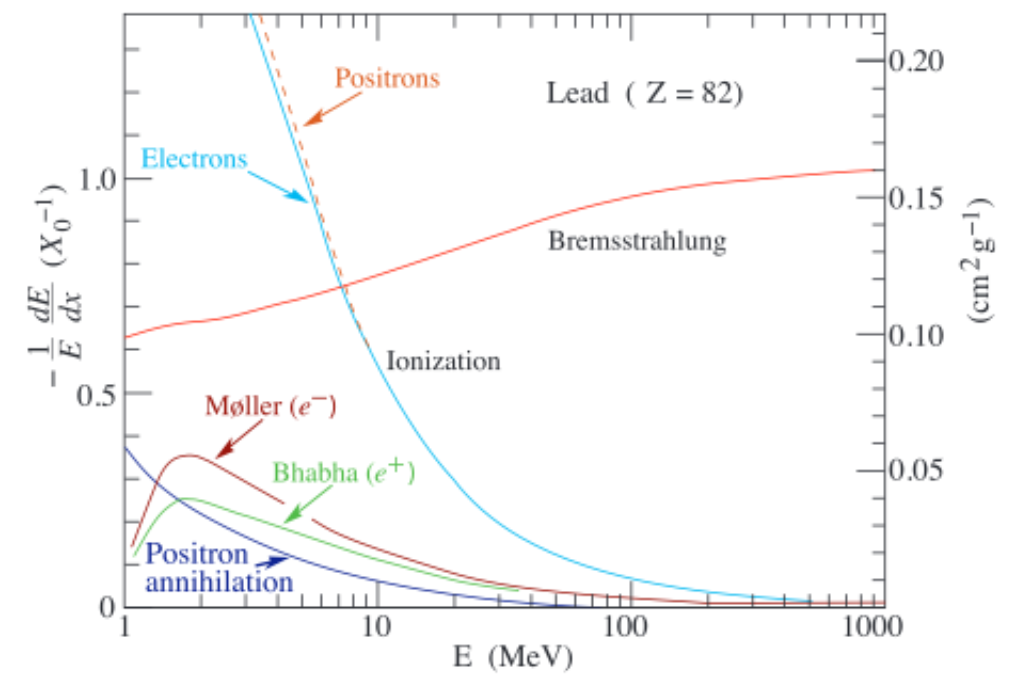
\includegraphics[width=10cm, keepaspectratio]{stoppingpower.png}
		\caption{Confronto dello stopping power per diversi tipi di radiazione nel piombo.}
         \label{stoppingpower}
\end{figure}


\section{Interazioni Fotoni-Materia}


Nelle interazioni tra fotoni e materia la probabilità che un quanto di luce interagisca con la materia in un trattino $\mathrm{d}x$ è effettivamente indipendente dal resto del cammino. Questa probabilità è proporzionale alla larghezza del trattino e dunque si può scrivere la seguente relazione:

\begin{equation}
\mathrm{d}p=\mu \mathrm{d}x
\end{equation}

Dove il coefficiente di proporzionalità $\mu$ viene chiamato coefficiente di assorbimento, e dipende dal tipo di interazione che sta avvenendo, nonché dall'energia del fotone incidente. Il numero di fotoni che vengono assorbiti in un tratto $dx$ allora sarà dato dalla seguente relazione:

\begin{equation}
\mathrm{d}N(x)=-N(x)\mu \mathrm{d}x
\end{equation}

Con soluzione

\begin{equation}
I(x)=I(0)e^{-\mu x}
\label{Intensity}
\end{equation}

Dove si è considerato che l'intensità di un fascio luminoso è proporzionale al numero di fotoni che compongono tale fascio.
In generale si possono avere più interazioni di vario tipo, con diverso coefficiente di assorbimento. Sommando i contributi di tale interazioni si ha che:

\begin{equation}
\mu=\sum \mu_{i}
\end{equation}

Introduciamo ora invece il concetto di sezione d'urto. 
La sezione d'urto è una grandezza prettamente sperimentale. In una schematizzazione classica in cui il fascio incidente incontra una serie di ostacoli che bloccano parte di tale fascio facendone passare il resto, la sezione d'urto rappresenta la superficie ostacolante costituita nel nostro caso dalle molecole del corpo umano. L'equazione differenziale che la definisce è la seguente:

\begin{equation}
\mathrm{d}\Phi(x)=-\sigma_{b}n_{b}\Phi(x)\mathrm{d}x
\end{equation}

Dove $\Phi$ è il flusso di particelle, $\sigma_{b}$ è la sezione d'urto del singolo elemento che compone il bersaglio, $n_b$ è la densità numerica di elementi con tale sezione d'urto inclusi nel bersaglio.

La soluzione di tale equazione differenziale risulta:

\begin{equation}
\Phi(x)=\Phi(0)e^{-\sigma_{b}n_{b}x}
\label{Flux}
\end{equation}

Confrontando le equazioni (\ref{Intensity}) e (\ref{Flux}), diverse solo per un coefficiente moltiplicativo (la superficie del fascio), otteniamo la seguente relazione tra coefficiente di assorbimento e sezione d'urto:

\begin{equation}
\mu=\sigma_{b} n_{b}
\end{equation}

\subsection{Effetto Fotoelettrico}

L'effetto fotoelettrico consiste nell'assorbimento da parte dell'atomo bersaglio di tutta l'energia del fotone incidente, che dunque si traduce nella ionizzazione di un elettrone che viene emesso con energia:

\begin{equation}
E_{e^-}=E_{\gamma}-I
\end{equation}

Dove $I$ è l'energia di ionizzazione dell'elettrone colpito. Tale fenomeno è dunque un effetto a soglia: avviene solamente se l'energia del fotone è maggiore a quella di ionizzazione dell'elettrone.

Si osserva sperimentalmente che la sezione d'urto dell'effetto fotoelettrico ha il seguente andamento dipendente dal bersaglio e dall'energia del fotone incidente:

\begin{equation}
\sigma_{photo}\simeq Z^5\alpha(\frac{m_{e}c^2}{E_{\gamma}})^n
\end{equation}

Dove $Z$ è il numero atomico del bersaglio, $\alpha$ è la costante di struttura fine, $n$ vale 3.5 o 1 a seconda che l'energia del fotone sia minore dell'energia a riposo dell'elettrone o ne sia molto maggiore. Nel caso in esame L'energia del fotone è al massimo di $100 keV$ mentre quella a riposo dell'elettrone è di $511 keV$ dunque va usato $n=3.5$.
Ricordando la relazione tra sezione d'urto e coefficiente di assorbimento posso ricavarne l'espressione:

\begin{equation}
\mu=n_{b}\sigma_{b} 
\end{equation}

\begin{equation}
\mu_{photo}\simeq\frac{\rho N_{A}}{A}Z^5\alpha(\frac{m_{e}c^2}{E_{\gamma}})^{3.5}
\end{equation}

\subsection{Effetto Compton}

L'effetto Compton è la descrizione del fenomeno per il quale un fotone in scattering elastico con un elettrone subisce una variazione di lunghezza d'onda. In tale processo la sua energia non è completamente assorbita dall'elettrone. Imponiamo la conservazione del quadriimpulso totale:

\begin{equation}
\gamma^{\mu}=(E_{\gamma},E_{\gamma}\hat{p_{\gamma}})\qquad e^{\mu}=(m_e,\vec{0}) \qquad \gamma'^{\mu}=(E'_{\gamma},E'_{\gamma}\hat{p'_{\gamma}}) \qquad e'^{\mu}=(E_e,\vec{p_e})
\end{equation}

\begin{equation}
e'^{\mu}=\gamma^{\mu}+e^{\mu}-\gamma'^{\mu}
\end{equation}

Facendo la norma quadra a sinistra e a destra ottengo

\begin{equation}
m_e^2=0+m_e^2+0+2\gamma^{\mu}e_{\mu}-2\gamma^{\mu}\gamma'_{\mu}-2\gamma'^{\mu}e_{\mu}=
\end{equation}
\begin{equation}
=m_e^2+2m_e(E_{\gamma}-E'_{\gamma})-2(E_{\gamma}E'_{\gamma}-E_{\gamma}E'_{\gamma}cos\theta)=
\end{equation}

Portando a sinistra ottengo
\begin{equation}
m_e(E_{\gamma}-E'_{\gamma})=E_{\gamma}E'_{\gamma}(1-cos\theta)
\end{equation}

\begin{equation}
\frac{1}{E'_{\gamma}}-\frac{1}{E_{\gamma}}=\frac{1-cos\theta}{m_e}
\end{equation}

Ora esplicitando l'energia finale del fotone che è ciò che ci interessa in questo caso otteniamo

\begin{equation}
E'_{\gamma}=\frac{E_{\gamma}m_e}{m_e+E_{\gamma}(1-cos\theta)}
\end{equation}

Da cui si osserva che il range di energie che prende il fotone è, per $\theta \in [0,\pi]$ $E'_{\gamma} \in [E_{\gamma},\frac{E_{\gamma}m_e}{m_e+2E_{\gamma}}]$

Imponendo semplicemente la conservazione della prima coordinata del quadriimpulso invece posso osservare il range di energie preso dall'elettrone:

\begin{equation}
E_{\gamma}+m_e=E'_{\gamma}+m_e+K'_e \qquad K'_e=E_{\gamma}-E'_{\gamma}
\end{equation}

Allora per l'energia cinetica dell'elettrone si può dire

\begin{equation}
K'_e \in [0, \frac{2E_{\gamma}^2}{m_e+2E_{\gamma}}]
\end{equation}

Sperimentalmente all'effetto Compton si associa la seguente sezione d'urto (elettroni non relativistici):

\begin{equation}
\sigma_{Compton}\simeq\frac{8\pi}{3}r_{e}^2
\end{equation}

Dove $r_{e}$ è il raggio classico dell'elettrone.

Da ciò ricaviamo il coefficiente di assorbimento Compton:

\begin{equation}
\mu_{Compton}\simeq\frac{\rho N_{A}}{A}Z\frac{8\pi}{3}r_{e}^2
\end{equation}

\subsection{Produzione di Coppie}

Quando un fotone ha abbastanza energia per produrre una coppia elettrone positrone (almeno la somma delle loro masse) esso può crearle a patto che vi sia un nucleo nelle vicinanze che può aiutare a bilanciare il quadriimpulso totale, che deve rimanere nullo in norma quadra come quello del fotone. 
Nella descrizione del fenomeno si considera nulla la variazione di energia cinetica del nucleo, e l'energia cinetica rispettivamente di elettrone e positrone è data dalla seguente uguaglianza:

\begin{equation}
K_{e^{+/-}}=\frac{E_{\gamma}-2m_e}{2}
\end{equation}

La sezione d'urto di tale fenomeno è:

\begin{equation}
\sigma_{pair-production}\simeq\frac{Z^2\alpha^3}{(m_ec^2)^2}
\end{equation}

Ricordando che $\mu=\sigma n$ e che $n=\frac{\rho N_A}{A}$:

\begin{equation}
\mu_{pp}=\frac{\rho N_A}{A}\frac{Z^2\alpha^3}{(m_ec^2)^2}
\end{equation}

La cosa importante da osservare è che tale assorbimento va con il quadrato del numero atomico.

\begin{figure}
\centering
		%% 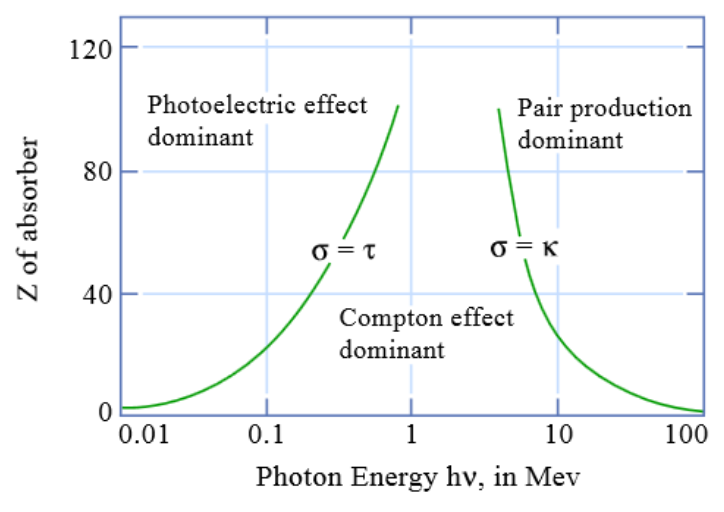
\includegraphics[width=10cm,keepaspectratio]{crosssection.png}
		\caption{Regioni di dominanza delle tre modalità di interazione dei fotoni con la materia, per diverse energie dei fotoni e diverso numero atomico dei bersagli.}
         \label{crosssection}
\end{figure}



\textbf{Terza Esperienza}

\emph{Stimare le quantità di piombo, plastica ($\text{C}_5\text{O}_2\text{H}_8$, $\rho=1,2 g/cm^3$) e paraffina ($\text{C}_{31}\text{H}_{64}$, $\rho=0,9 g/cm^3$) necessarie ad attenuare di un fattore di $10^{-4}$ dei fotoni o fermare elettroni e particelle alfa di energie $0.1$, $1$ e $10$ $MeV$.}

\section{Interazioni Positroni-Materia}

Il positrone prodotto in un decadimento $\beta+$ interagisce in primis per multiple scattering e ionizzazione. Dopodichè esso può fare due cose:

\begin{itemize}
\item Col $20\%$ di probabilità fa annichilazione in volo con un elettrone producendo due fotoni. Ponendoci nel sistema di riferimento dell'elettrone che viene colpito vale la relazione $2m_e+K_e=E_{\gamma1}+E_{\gamma2}$ e l'angolo tra i fotoni è minore di \ang{180}.
\item Con 80\% di probabilità comincia ad orbitare intorno ad un elettrone libero, formando il sistema $e^+e^-$ detto \emph{positronio}.
\end{itemize}

Analizziamo la possibilità della formazione del positronio. Esso a seconda dello spin totale forma l'orto-positronio o il para-positronio. Siccome lo stato di singoletto è uno solo mentre quelli di tripletto sono tre, la formazione di para-positronio (spin totale:$1$)è tre volte più probabile di quella dell'orto-positronio (spin totale:$0$). 
In totale per ogni decadimento che produce un positrone la probabilità di formare para-positronio è 64\%. 
Il para-positronio ha una vita media di $125 ps$ e poi decade in una coppia di fotoni back to back, mentre l'orto-positronio ha una vita media di $140 ns$ e decade in tre fotoni. La coppia di fotoni emessa dal para-positronio è interessante perché se rilevata può dare informazioni per triangolare dove è avvenuto il decadimento. Essi sono emessi a $\ang{180}$ per conservazione della quantità di moto. Inoltre, per conservazione dell'energia, i due fotoni sono esattamente da $511 keV$.
Proprio su questi principi si basa la PET, che per immissione di un radiofarmaco metabolico che decade $\beta+$, triangolando i fotoni, permette di fare diagnostica funzionale.
Il limite principale della PET è il fatto che i positroni prima di formare positronio si muovono nel corpo per scattering multiplo e ionizzazione, variando la loro posizione e dunque creando un incertezza sulla misura finale.
Risoluzione massima: $0,44 mm$.

Approfondimenti e bibliografia: \cite{PET1} \cite{PET2}

